\begin{table}[H]
\centering
\begin{tabular}{@{}lll@{}}
\toprule
\textbf{Aspecto} & \textbf{Axión} & \textbf{Electrón} \\ \midrule
Masa & \(10^{-5}\) eV & 511 keV \\
Longitud de onda & \(0,124\) m & \(2,4\times10^{-12}\) m \\
Comportamiento & Onda & Partícula \\
Interacción & Muy débil & Electromagnética \\
Papel en ART-12D & Modo del campo akáshico & Receptor neuronal \\ \bottomrule
\end{tabular}
\end{table}

\subsection{¿Qué partículas atraviesan su cuerpo?}
La materia oscura tiene una densidad local de aproximadamente 0,3 GeV/cm$^3$ (Read, 2014). La densidad numérica depende, sin embargo, de la masa, $n = \rho/m$, y el flujo es $\Phi = n v$. Para un modo de $10^{-5}$ eV y $v = 300$ km/s resulta:
\begin{equation}
n = \frac{0,3 \times 10^{15}\ \text{eV/m}^3}{10^{-5}\ \text{eV}} = 3,0\times10^{19}\ \text{m}^{-3},
\qquad
\Phi = n v = 9,0\times10^{24}\ \text{m}^{-2}\text{s}^{-1}.
\end{equation}
Para un cuerpo humano con una superficie de 0,7 m$^2$:
\begin{equation}
\Phi_{\text{body}} = 9,0\times10^{24} \times 0,7 \approx 6\times10^{24} \text{ particles/s}.
\end{equation}
Unos $6\times10^{24}$ partículas por segundo. (La versión 30 afirmaba $n = 3000$ m$^{-3}$ y $6\times10^8$ s$^{-1}$; esos valores corresponden a un WIMP de unos 100 GeV, no a un modo de $10^{-5}$ eV.)

\begin{figure}[H]
\centering
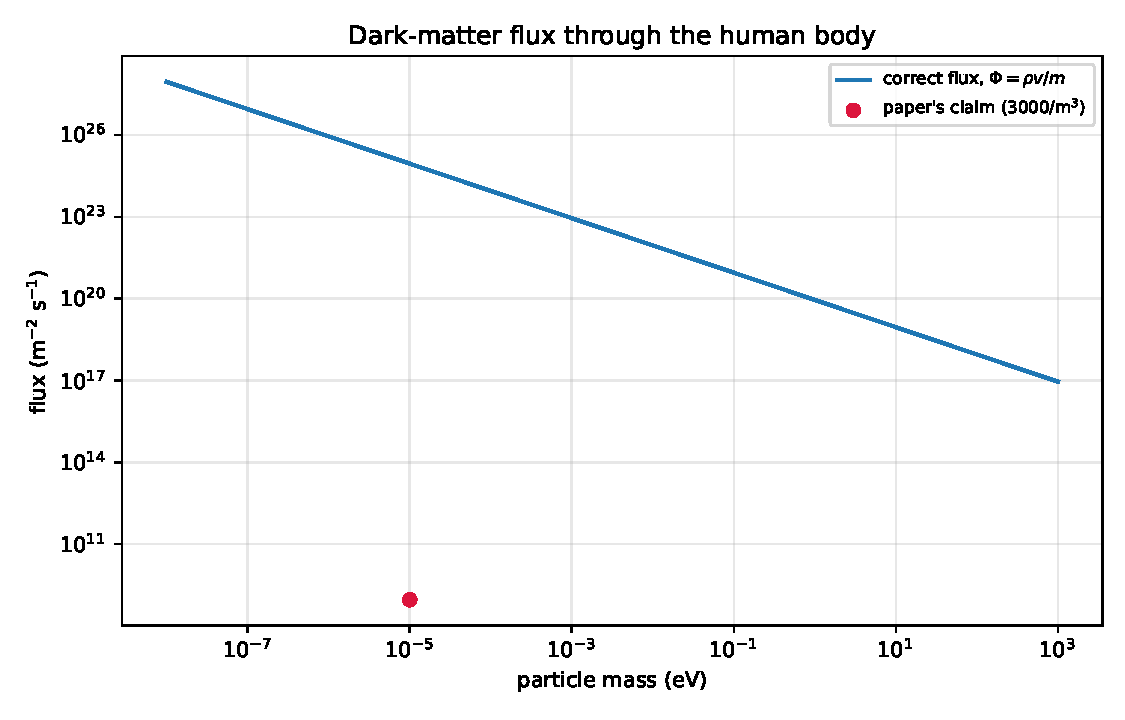
\includegraphics[width=0.82\textwidth]{figures/fig07_flux.pdf}
\caption{El flujo de materia oscura a través del cuerpo humano en función de la masa de la partícula. El punto rojo marca la afirmación de la versión 30; la curva es el valor correcto para $\rho = 0,3$ GeV/cm$^3$ y $v = 300$ km/s. A $10^{-5}$ eV la diferencia es de 16 órdenes de magnitud.}
\label{fig:flux}
\end{figure}

\subsection{¿Qué ocurre con esas partículas?}
La mayoría lo atraviesan sin interactuar. Algunas interactúan con los núcleos atómicos: independiente del espín ($\sim 5$ colisiones/año), dependiente del espín ($\sim 30$ colisiones/año). El efecto sobre el cuerpo: radiación natural ($\sim 2,4$ mSv/año); materia oscura ($\sim 10^{-15}$ mSv/año).

\subsection{¿Cómo detectamos esas partículas?}
Detectores directos: LUX-ZEPLIN (10 toneladas de xenón) --- sensibilidad: $10^{-48}$ cm$^2$. Detectores indirectos: Fermi-LAT (busca rayos gamma de aniquilación), ADMX (busca axiones). Sección eficaz: $\sigma \sim 10^{-47}$ cm$^2$. Probabilidad de interacción: $P \sim 10^{-22}$.

\subsection{La materia oscura como onda, no como partículas}
Si la materia oscura es un campo escalar, no está compuesta de partículas individuales. Es una onda que llena el universo. Formalización: $A(x,t) = \sum_n A_n \cos(\omega_n t + \varphi_n)$.

\subsection{La analogía del árbol y el fotón}
Imagine un árbol en una playa. El sol brilla. Los fotones salen del sol con energía $E = h\nu$. Llegan al árbol. Son absorbidos por cada hoja con la misma energía $h\nu$. ¿Cómo puede un solo fotón llegar a todas las hojas con la misma energía? Si fuera una partícula, perdería energía en cada colisión. Pero no lo hace. La respuesta es sencilla: porque el fotón es una onda, no una partícula. Una onda no se «consume» al atravesar la materia. Se extiende por todo el espacio. Cada hoja «ve» la onda entera. El estado del fotón: $|\psi_{\text{photon}}\rangle = \int d^3k \, c(k) |k\rangle$.

\subsection{La dualidad onda--partícula como mecanismo de travesía}
Si la materia no puede atravesar entre universos (porque requeriría energía infinita) y los universos están conectados por la materia oscura, ¿cómo se comunican? La respuesta ART-12D: mediante la dualidad onda--partícula. Etapa 1: la materia se convierte en onda. $|\text{particle}\rangle_A \to |\text{wave}\rangle_A$. Etapa 2: la onda atraviesa. $|\text{wave}\rangle_A \to |\text{wave}\rangle_B$. Etapa 3: la onda se convierte en partícula. $|\text{wave}\rangle_B \to |\text{particle}\rangle_B$. Etapa 4: la información se transduce. $I_A \to I_B$.

\subsection{El espectro emocional humano}
Los sentimientos humanos se dividen en dos grandes categorías: positivos y negativos. Cada sentimiento tiene una frecuencia característica y un efecto específico sobre la conciencia. Formalización: $S_{\text{total}} = \sum_{i=1}^{48} S_i^{\text{positive}} + \sum_{j=1}^{46} S_j^{\text{negative}}$. He aquí un extracto de la tabla ampliada (la versión completa figura en el anexo B):
\begin{table}[H]
\centering
\begin{tabular}{@{}lll@{}}
\toprule
\textbf{Sentimiento} & \textbf{Frecuencia dominante (Hz)} & \textbf{Efecto} \\ \midrule
Alegría & 400-600 & Expansión, dinamismo \\
Paz & 200-350 & Calma reflexiva \\
Amor & 200-400 & Emoción profunda \\
Gratitud & 300-500 & Satisfacción \\
Miedo & 500-800 & Activa la amígdala \\
Ira & 600-800 & Rabia \\
Tristeza & 400-600 & Melancolía \\
Envidia & 600-800 & Celos \\ \bottomrule
\end{tabular}
\end{table}
Las frecuencias musicales terapéuticas (432 Hz, 528 Hz, 639 Hz, 741 Hz, 852 Hz, 963 Hz) se han correlacionado con las frecuencias del campo akáshico. Los siete sentidos humanos comprenden cinco físicos (vista, oído, olfato, gusto, tacto) y dos psíquicos (imaginación, empatía).

\subsection{El corazón como modulador de la recepción}
El corazón posee un sistema eléctrico propio (el nódulo sinoauricular) que genera impulsos con independencia del cerebro. Funciona como un modulador de la recepción, no como un receptor independiente. El cerebro es el receptor principal, el corazón ajusta la coherencia. Formalización: $C_{\text{coherent}} = C_0 \times (1 + \beta \times HRV)$. Las cifras científicas exactas: el cerebro consume unos $20$ W de potencia metabólica, el corazón entrega unos $1-1,3$ W de potencia mecánica, pero produce campos eléctricos y magnéticos de amplitud mucho mayor.

\subsection{La palabra que puede sustituir a cualquier medicamento}
La hipótesis: $L_{\text{word-matter}} = g_{CM} A_{\text{meaning}} \psi \psi$. Lo que la palabra puede hacer: $Effect_{\text{total}} = Effect_{\text{medicine}} + Effect_{\text{word}} + \text{Interaction}$. Lo que la palabra no puede hacer: no puede sustituir a los antibióticos en las infecciones bacterianas, no puede sustituir a la insulina en la diabetes tipo 1, no puede sustituir a la cirugía en la apendicitis, no puede sustituir a la quimioterapia en el cáncer. Predicción 67: el efecto de la palabra.

\newpage
